% Copyright 2004 by Till Tantau <tantau@users.sourceforge.net>.
%
% In principle, this file can be redistributed and/or modified under
% the terms of the GNU Public License, version 2.
%
% However, this file is supposed to be a template to be modified
% for your own needs. For this reason, if you use this file as a
% template and not specifically distribute it as part of a another
% package/program, I grant the extra permission to freely copy and
% modify this file as you see fit and even to delete this copyright
% notice. 

\documentclass{beamer}

% There are many different themes available for Beamer. A comprehensive
% list with examples is given here:
% http://deic.uab.es/~iblanes/beamer_gallery/index_by_theme.html
% You can uncomment the themes below if you would like to use a different
% one:
%\usetheme{AnnArbor}
%\usetheme{Antibes}
%\usetheme{Bergen}
%\usetheme{Berkeley}
%\usetheme{Berlin}
%\usetheme{Boadilla}
%\usetheme{boxes}
%\usetheme{CambridgeUS}
%\usetheme{Copenhagen}
%\usetheme{Darmstadt}
%\usetheme{default}
%\usetheme{Frankfurt}
%\usetheme{Goettingen}
%\usetheme{Hannover}
%\usetheme{Ilmenau}
%\usetheme{JuanLesPins}
%\usetheme{Luebeck}
\usetheme{Madrid}
%\usetheme{Malmoe}
%\usetheme{Marburg}
%\usetheme{Montpellier}
%\usetheme{PaloAlto}
%\usetheme{Pittsburgh}
%\usetheme{Rochester}
%\usetheme{Singapore}
%\usetheme{Szeged}
%\usetheme{Warsaw}


% Customize Warsaw color 
\setbeamercolor*{palette primary}{use=structure,fg=white,bg=red!50!black}
\setbeamercolor*{palette secondary}{use=structure,fg=white,bg=red!60!black}
\setbeamercolor*{palette tertiary}{use=structure,fg=white,bg=red!70!black}

% Customize Warsaw block title and background colors
\setbeamercolor{block title}{bg=red!50!black,fg=white}


% List your packages here

\usepackage[colorinlistoftodos]{todonotes}


\title[Progress]{BEMOSS and Its Enhanced Applications}

% % A subtitle is optional and this may be deleted
% \subtitle{Product Proposal}

\author[B.~Lauer]{Brian~Lauer \\\and
Advisor: Dr. Suruz Miah}
% - Give the names in the same order as the appear in the paper.
% - Use the \inst{?} command only if the authors have different
%   affiliation.

\institute[Bradley University] % (optional, but mostly needed)
{
  Department of Electrical and Computer Engineering\\
  Bradley University\\
  1501 W. Bradley Avenue\\
  Peoria, IL, 61625, USA
}
% - Use the \inst command only if there are several affiliations.
% - Keep it simple, no one is interested in your street address.

\date[August~2,~2019]{Friday, August~2,~2019}
% - Either use conference name or its abbreviation.
% - Not really informative to the audience, more for people (including
%   yourself) who are reading the slides online

\logo{\hfill\href{http://www.bradley.edu}{
\includegraphics[width=0.75cm]{figs/logoBU1-Print}}}  % place logo in every page 


\subject{Mobile Robot Localization}
% This is only inserted into the PDF information catalog. Can be left
% out. 

% If you have a file called "university-logo-filename.xxx", where xxx
% is a graphic format that can be processed by latex or pdflatex,
% resp., then you can add a logo as follows:

% \pgfdeclareimage[height=0.5cm]{university-logo}{university-logo-filename}
% \logo{\pgfuseimage{university-logo}}

% Delete this, if you do not want the table of contents to pop up at
% the beginning of each subsection:
\AtBeginSubsection[]
{
  \begin{frame}<beamer>{Outline}
    \tableofcontents[currentsection,currentsubsection]
  \end{frame}
}




% Let's get started
\begin{document}

\begin{frame}
  \titlepage
\end{frame}

\begin{frame}{Outline}
  \tableofcontents
  % You might wish to add the option [pausesections]
\end{frame}

%----------------------------------
\section{VOLTTRON}

\begin{frame}{VOLTTRON}
	\begin{columns}
		\begin{column}{0.5\textwidth}
		\begin{figure}
			\centering
			
\includegraphics[scale=0.15]{figs/volttronlogo.png}
			\caption{Source https://volttron.readthedocs.io/}
		\end{figure}
		\end{column}
		\begin{column}{0.5\textwidth}
			\begin{block}{Overview}
			\begin{itemize}
			\item Agent-based system for improving energy management
			\item Improves sensing and control of devices in buildings
			\item Single point of contact for interfacing with devices (RTUs, building systems, power meters)
			\item Open source, available on github
			\item Python 2.7, Linux
			\end{itemize}
			\end{block}
		\end{column}
	\end{columns}
\end{frame}

\begin{frame}{VOLTTRON}
\begin{figure}
\centering
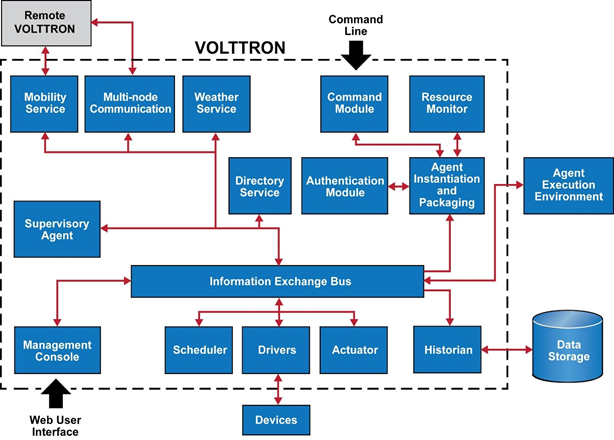
\includegraphics[scale=0.5]{figs/volttronoverview.png}
%\caption{Source: https://volttron.readthedocs.io/}
\end{figure}
\end{frame}

\section{Motor Interface}

\begin{frame}{Motor Interface}
\begin{block}{Update}
\begin{itemize}
\item Added identify device behavior to motor
\item Python Digi-XBee library instead of python-xbee library
\begin{itemize}
	\item Commands to read status of IO pins
	\item Send commands to end point XBee specifying remote node identification
\end{itemize}
\end{itemize}
\end{block}
\end{frame}

\begin{frame}{Motor Interface}
\begin{figure}
\centering
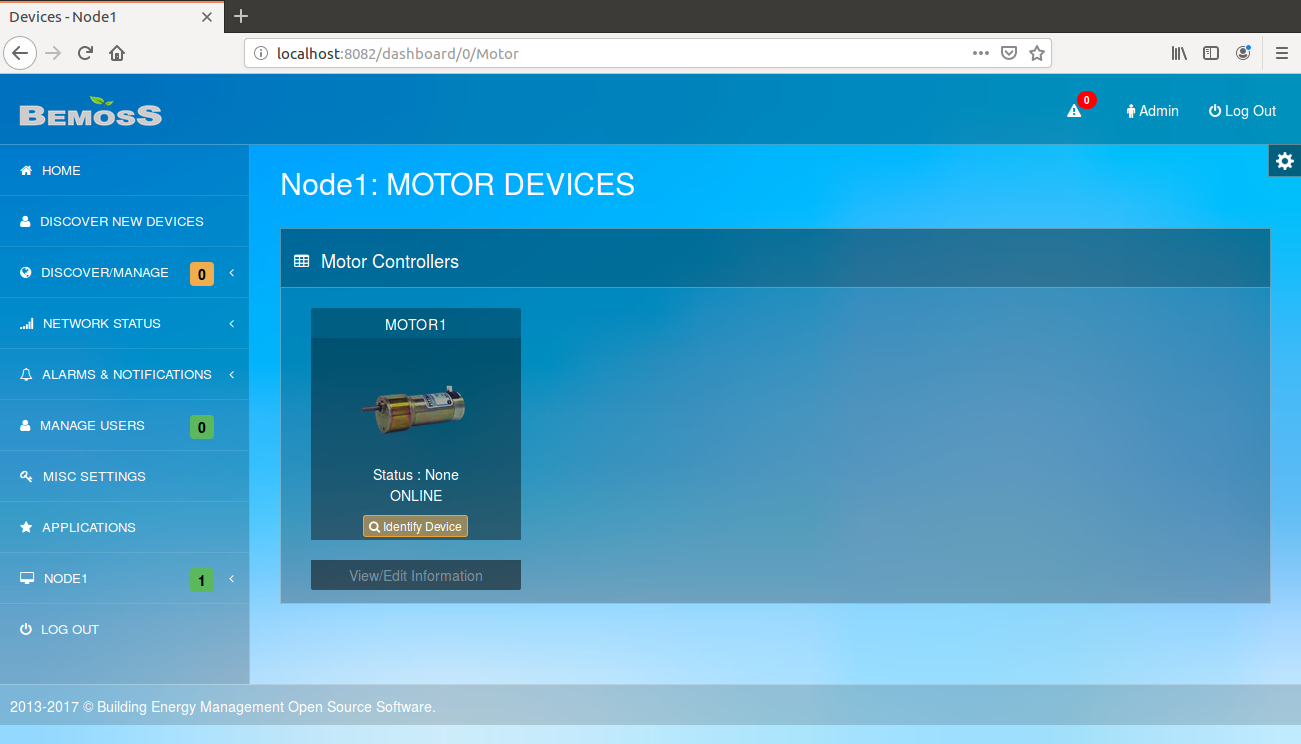
\includegraphics[scale=0.25]{figs/motordevices.png}
\end{figure}

\end{frame}

\begin{frame}{Motor Interface}
\begin{block}{Problems}
\begin{itemize}
\item No chart visible
\item Motor not properly added to BEMOSS database (PostgreSQL)
\begin{itemize}
\item Required to run \texttt{PROJECT\_DIR/Web\_Server/run/defaultDB.py}
\end{itemize}
\end{itemize}
\end{block}
\end{frame}

\begin{frame}{Motor Interface}
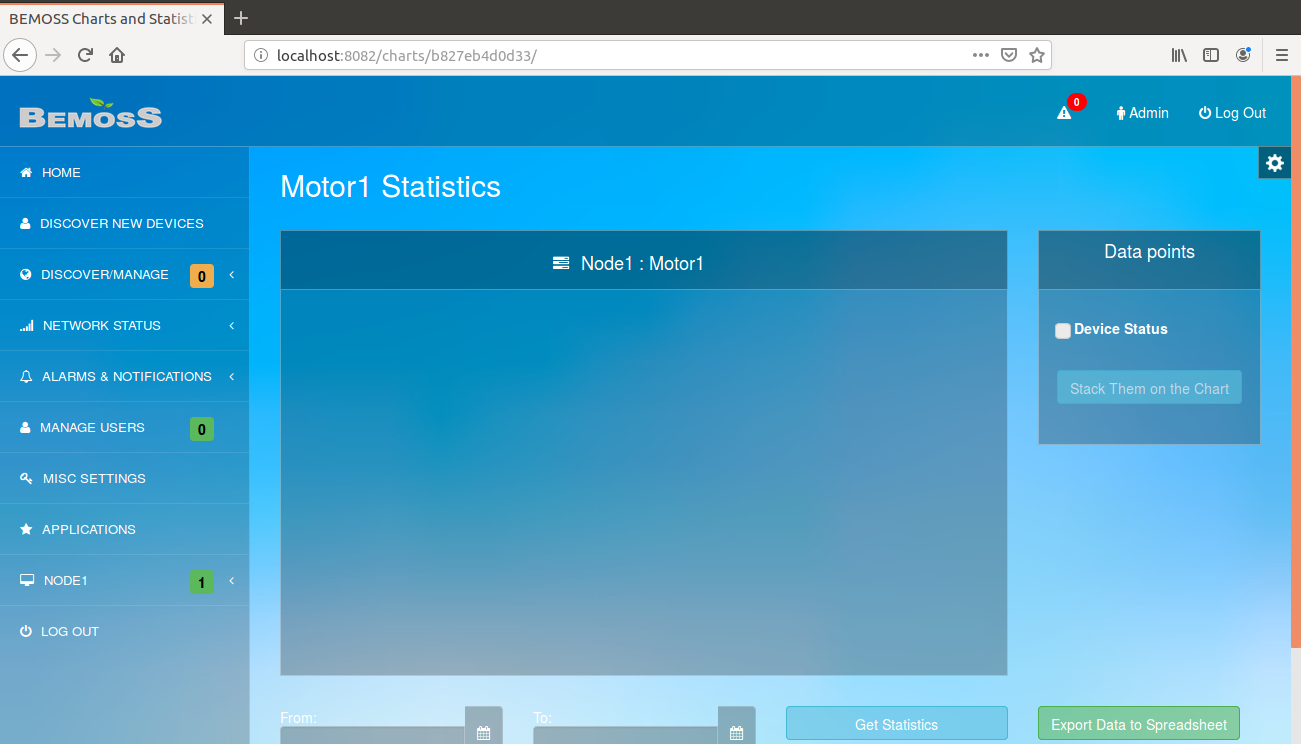
\includegraphics[scale=0.25]{figs/nomotorchart.png}
\end{frame}

\section{Bug Fixes}

\begin{frame}{Bug Fixes}
\begin{block}{Corrected TSDAgent Error}
\begin{itemize}
\item Downgraded Python cassandra-driver to version 3.16.0
\end{itemize}
\end{block}
\end{frame}

\section{Plans}

\begin{frame}{Plans}
\begin{block}{Finish motor interface}
\begin{itemize}
\item Fix database and chart issues
\item Implement ssh keys
\end{itemize}
\end{block}
\begin{block}{Begin writing paper}
\begin{itemize}
	\item Motor interface must be fully functional
\end{itemize}
\end{block}
\begin{block}{Develop deep understanding of BEMOSS}
	\begin{itemize}
		\item Understand every part of the code base
		\begin{itemize}
			\item This is required to make further progress
		\end{itemize}
		\item Completed before August 23
	\end{itemize}
\end{block}
\begin{block}{Add new device}
\begin{itemize}
\item Possibly space heater
\end{itemize}
\end{block}
\end{frame}
\begin{frame}{Plans}
\begin{figure}
	\centering
	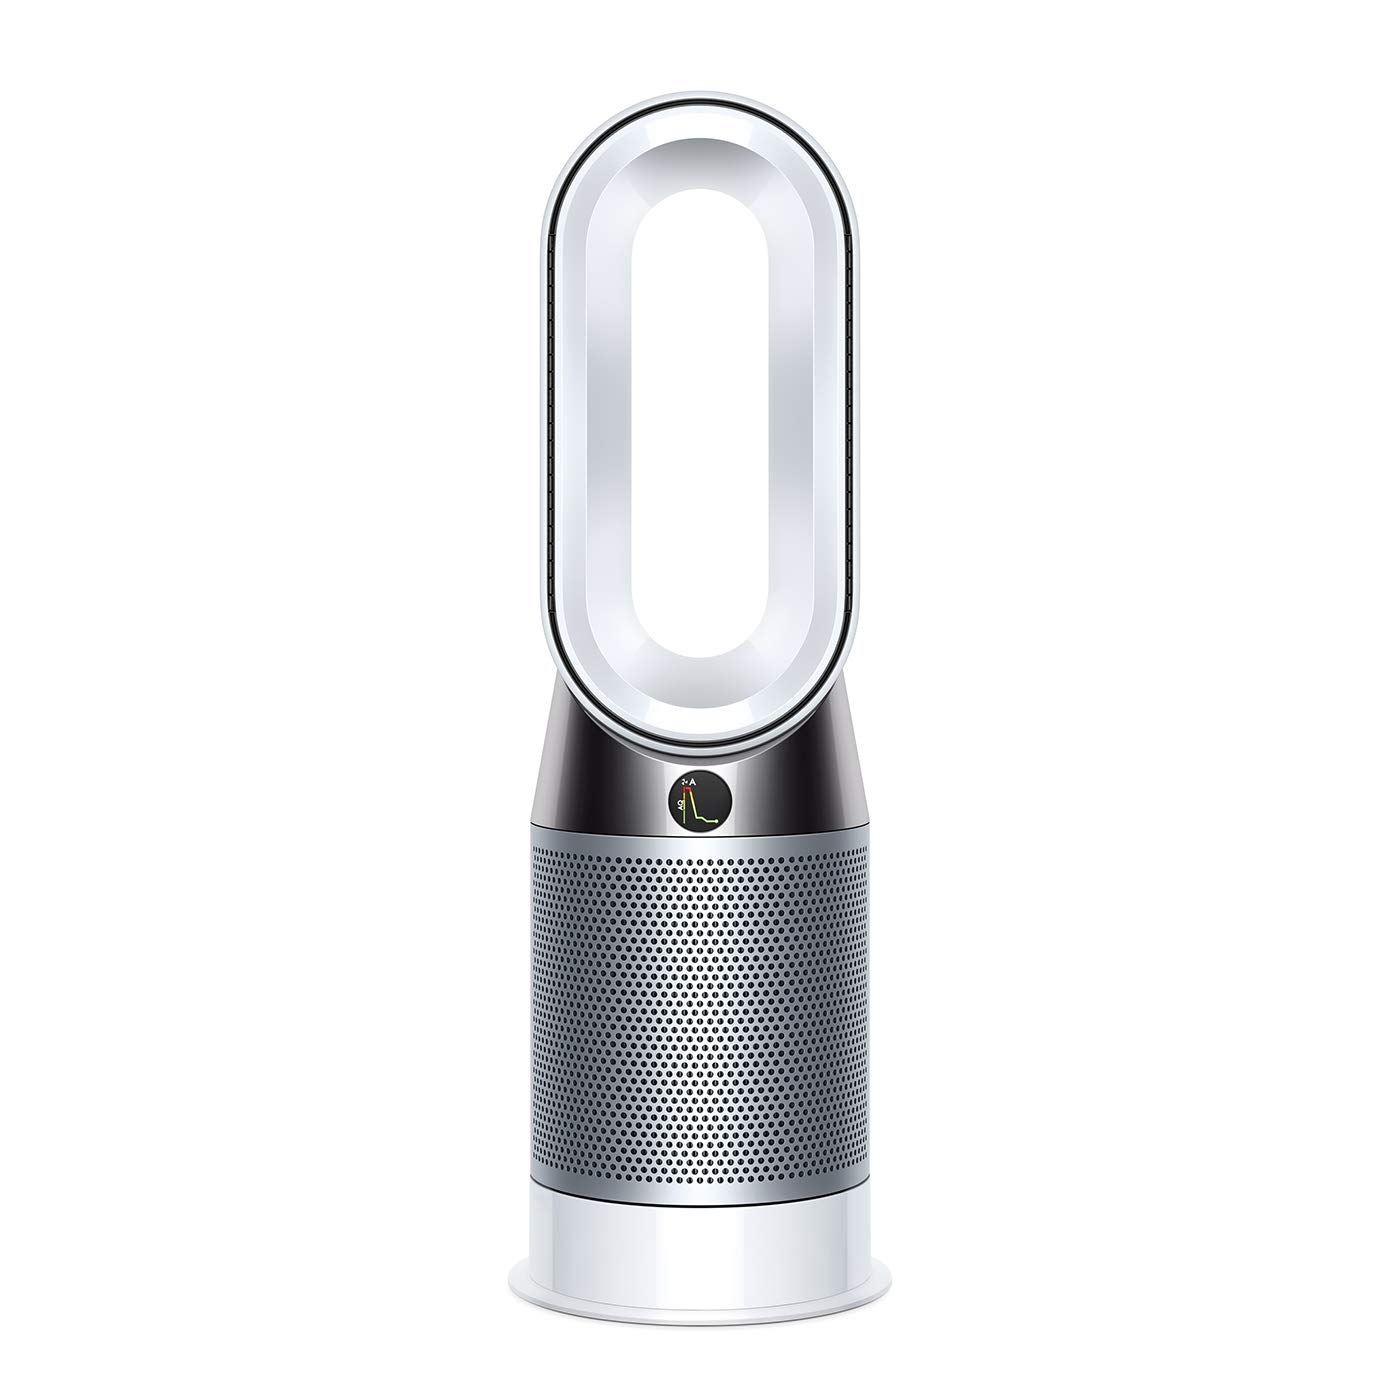
\includegraphics[scale=0.11]{figs/dysonairpurifier.jpg}
	\caption{Dyson Pure Hot + Cool Air Purifier Courtesy of https://www.wantse.com/images/2/o6y516bzd.jpg}
\end{figure}
\end{frame}

% All of the following is optional and typically not needed. 
\appendix
\section<presentation>*{\appendixname}
\subsection<presentation>*{For Further Reading}

\begin{frame}[allowframebreaks]
  \frametitle<presentation>{For Further Reading}
    
  \begin{thebibliography}{10}
   
  \setbeamertemplate{bibliography item}[online]

  \bibitem{volttrondocs}
    VOLTTRON
    \newblock VOLTTRON Documentation.
    \newblock \texttt{https://volttron.readthedocs.io/}
    
  \end{thebibliography}
\end{frame}

\end{document}



%%% Local Variables:
%%% mode: latex
%%% TeX-master: t
%%% End:
